\chapter{Research methodology} 

This work focuses on three parameters, which are important for the brake bending. Springback, bend deduction and edge cracking. 
The following describes the experimental setup used for the experiments performed. 

\section{Dataset generation} 
For the dataset generation bending experiments were performed on metal sheets with different thickness. 
% material
The material used is cold rolled steel sheets of the norm DIN EN 10130. The thicknesses used were 0.5mm, 1mmm and 2mm. 
The material was used because it is commonly used in bending processes and its high availability. In previous tests, it was observed, that the spring back and bend deduction are well observable with this material. 
Using this material, 200 single bending pieces of the dimension 50×100 mm have been cut. 
Each piece was bend one time using a \textit{XXXX} brake bending machine. The bend parts where digitalized using a scanner and the resulting images were measured with image processing software ImageJ. 

\subsection{Measurement of the parameters}
The two main parameters in the dataset are the \textit{spring back} and the \textit{bend deduction}. 
The following describes how these were measured and possible limitations of the used methods. 

\paragraph{Springback:}
The brake bending machine used for the experimental setup was set to an angle. After the bending operation, the metal sheet sprung back. To get the spring back, the angle after the bend was measured with a protractor and subtracted from the angle, that was set in the machine. The angle was measured another time digitally using the \textit{ImageJ} software to minimize the margin of error.

\paragraph{Bend deduction:}
Measuring the bend deduction is more complex. After a metal sheet is bent, it is hard to measure the flat pattern length because the material is malformed at the bent. 
As a result, the neutral axis is not in the center of the sheet and hard to measure, but it can be calculated using different approaches. %quelle und ausführlicher und grunlagen teil  
There are multiple ways to measure the bend deduction described earlier. 
% K-Faktor Muss noch in theorie teil 
In this setup, the method described in the DIN6395 was used. This method uses a k-factor which is an approximated value and therefore and therefore it can be inaccurate. (Equation~\ref{eq:kfactor}). % cite DIN norm 

\begin{equation}\label{eq:kfactor}
    k=0.65+\frac{1}{2}\log{\frac{r}{s}}
\end{equation}

\begin{figure}[ht!] % supposedly places it here ...
	\centering
	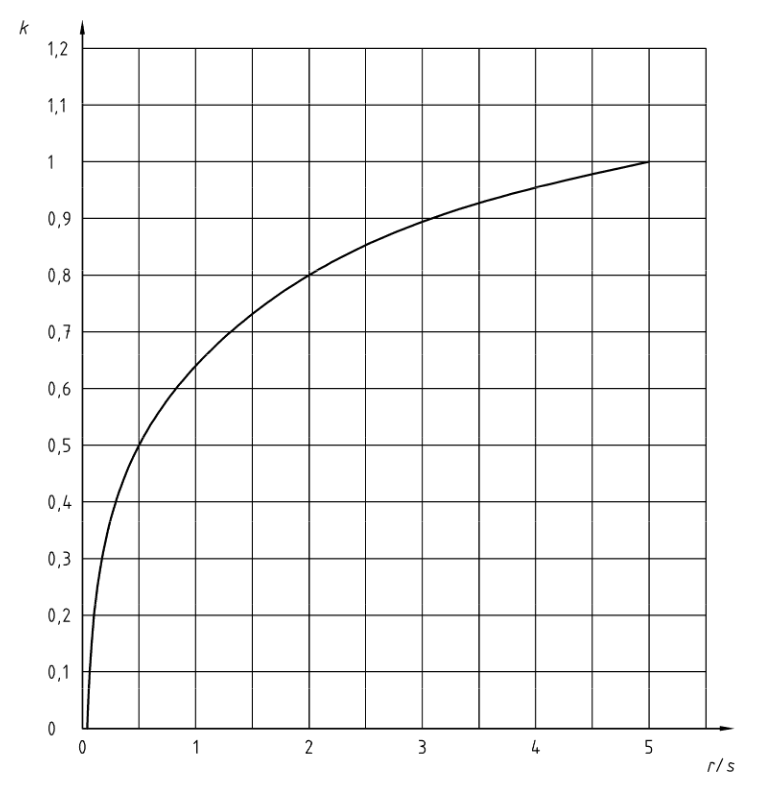
\includegraphics[width=0.5\linewidth]{k-factor}
	\caption[Graphical representation of the correction factor]{Graphical representation of the correction factor.}
	\label{fig:test1}
\end{figure}

The DIN 6935 used the formula for the stretched length, $length=a+b+v$ where \textit{a} and \textit{b} are the side lengths of the sheet and \textit{v} is a correction value for the deduction. \cite{din6935}
The stretched length is measured different depending on the bending angle.

\paragraph{Opening angle $\beta 0^\circ$ to $90^\circ$} 
For opening angles between $0^\circ$and $90^\circ$ the side lengths \textit{a} and \textit{b} are dimensioned from the tangent of the bend to the edge. 
To calculate the compensation value \textit{v} (Equation~\ref{eq:v1}) is used
\cite{din6935}.

\begin{equation}\label{eq:v1}
        v=\pi*(\frac{180^\circ-}{180^\circ})*(r+\frac{s}{2}*k)-2(r+s)
\end{equation}

\begin{figure}[H]
	\centering
	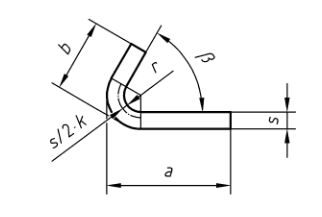
\includegraphics[width=0.5\linewidth]{bending-angle-90}
	\caption[Opening angles $\beta 0^\circ$ to $90^\circ$]{Opening angles $\beta 0^\circ$ to $90^\circ$ \cite{din6935}}
	\label{fig:v1-image}
\end{figure}

\paragraph{Bending angle $\beta90^\circ$ to $165^\circ$} (Equation~\ref{eq:v1})
For opening angles between $90^\circ$ and $165^\circ$ the side lengths \textit{a} and \textit{b} are dimensioned from the apex to the edge. 
To calculate the compensation value \textit{v} (Equation~\ref{eq:v1}) is used. 
\cite{din6935}

\begin{equation}\label{eq:v2}
    v=\pi*(\frac{180^\circ-}{180^\circ})*(r+\frac{s}{2}*k)-2(r+s)+\tan{\frac{180^\circ-\beta}{2}}
\end{equation}

\begin{figure}[!h]
	\centering
	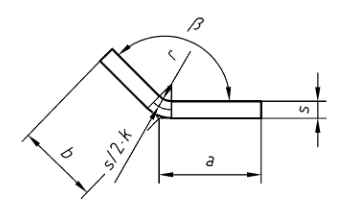
\includegraphics[width=0.5\linewidth]{bending-angle-165}
	\caption[Opening angles $\beta90^\circ$ to $165^\circ$]{Opening angles $\beta90^\circ$ to $165^\circ$ \cite{din6935}}
	\label{fig:v2-image}
\end{figure}

For opening angles between $165^\circ$ and $180^\circ$ the compensation value \textit{v} is 0. The values for v would be negligibly small. \cite{din6935} The side lengths \textit{a} and \textit{b} where measured using the software \textit{ImageJ}. 

Edge cracking is not measured for now because the steel used has no high-strength and with machine in usage it was not possible to create edge cracking.

\begin{figure}[!h]
	\centering
	\includegraphics[width=0.5\linewidth]{example-image}
	\caption[Screenshot ImageJ]{Screenshot ImageJ}
	\label{fig:imagej-screenshot}
\end{figure}



\begin{table}[ht!]
\centering
    \begin{tabular}{ |c|c|c|c| } 
        \hline
        Parameters & Mechanical Press \\
        \hline
        Load Tonnage (T) & tbd... \\
        Material & JSC440, JSC590, JSH440, JSH590 \\
        Thickness of blank (s) & 1.0 mm, 1.2 mm, 1.4 mm, 1.6 mm \\ 
        dimensions of plate (w) & 50 mm, 100 mm \\ 
        Bend angle & 60, 90 and 120 \\
        \hline
    \end{tabular}
    \caption{Parameters for the experimental setup}
\end{table}

